\documentclass{article}

\usepackage[utf8]{inputenc}
\usepackage[T1]{fontenc}
\usepackage{amsmath}
\usepackage{listings}
\usepackage{graphicx}
\inputencoding{utf8}

\title{Rapport de TP : Développement d'un module de table de hachage en Python}
\author{Wolodia ZDETOVETZKY}
\date{03/2023}


\begin{document}

    \maketitle
    \tableofcontents
    \newpage

    \section{Introduction}\label{sec:introduction}

    L'utilisation de structures de données efficaces est un élément clé dans le développement d'applications performantes en informatique.
    Parmi les nombreuses structures de données existantes, les tables de hachage sont largement utilisées en raison de leur efficacité en termes de temps d'accès aux données.
    Dans cette étude, nous nous concentrerons sur le développement d'un module de table de hachage en Python.
    Les tables de hachage sont une structure de données qui permet de stocker et d'accéder rapidement à des valeurs à partir d'une clé.
    L'objectif principal des tables de hachage est de fournir une fonction de hachage efficace qui permet de calculer un index de tableau à partir d'une clé.
    Le processus de hachage consiste à appliquer une fonction de hachage à une clé pour calculer un index, qui est ensuite utilisé pour accéder à la valeur correspondante.

    Les tables de hachage sont particulièrement adaptées pour stocker des données de grande taille et sont souvent utilisées dans les bases de données, les systèmes de gestion de fichiers et les applications de recherche.
    Les tables de hachage ont également l'avantage de pouvoir être utilisées pour résoudre des problèmes de recherche et de filtrage en temps constant.

    Cependant, les tables de hachage présentent également certaines limites.
    Tout d'abord, les collisions peuvent se produire lorsqu'il y a deux clés différentes qui se retrouvent avec le même index.
    Cela peut ralentir les performances de la table de hachage.
    De plus, les tables de hachage ont une taille fixe, ce qui signifie qu'elles ne peuvent pas être agrandies une fois qu'elles sont créées.

    Dans ce rapport, nous présentons le développement d'un module de table de hachage en Python qui offre un type abstrait Table.
    Le module se base sur une implémentation de table de hachage avec des collisions résolues par adressage fermé puis ouvert.
    La taille de la table est fixe et l'utilisateur peut choisir entre plusieurs fonctions de hachage et méthodes de rehachage.
    Le module offre également des méthodes d'insertion, de suppression, de recherche, d'union et d'intersection de tables ainsi qu'une méthode d'affichage.

    Nous présentons aussi une analyse des performances de notre module de table de hachage en fonction de la taille de la table, du nombre d'insertions et de recherche d'une clé.
    Nous comparons les performances de notre module avec d'autres structures de données et implémentations.

    Dans les sections suivantes, nous détaillons l'implémentation de notre module de table de hachage en Python, les tests de performances effectués ainsi que l'analyse de la complexité algorithmique de notre implémentation.

    \newpage
    \section{Présentation du sujet}\label{sec:presentation}

    Le sujet de ce rapport est le développement d'un module de table de hachage en Python.
    L'objectif est de créer un type abstrait Table en utilisant une implémentation de table de hachage, où la clé sera un entier et la taille de la table sera fixe.

    Le module devra offrir plusieurs méthodes pour la manipulation des tables de hachage :
    \begin{itemize}
        \item \texttt{init(taille\_table, fonction\_hachage, type\_rehachage)} - cette méthode initialisera la table de hachage en spécifiant la taille de la table, la fonction de hachage à utiliser et le type de rehachage (linéaire, quadratique ou double hachage).
        \item \texttt{insert(key, value)} - cette méthode insérera une paire clé-valeur dans la table.
        \item Si la clé existe déjà dans la table, la valeur associée sera mise à jour.
        \item \texttt{delete(key)} - cette méthode supprimera la paire clé-valeur associée à la clé spécifiée de la table.
        \item \texttt{exist(key)} - cette méthode renverra True si la clé spécifiée existe dans la table, False sinon.
        \item \texttt{value(key)} - cette méthode renverra la valeur associée à la clé spécifiée.
        \item \texttt{union(autre\_table)} - cette méthode renverra une table résultant de l'union de la table actuelle avec une autre table spécifiée en argument.
        \item \texttt{intersection(autre\_table)} - cette méthode renverra une table résultant de l'intersection de la table actuelle avec une autre table spécifiée en argument.
        \item \texttt{affichage()} - cette méthode affichera les éléments insérés dans la table ainsi que le nombre de rehachage nécessaire pour chaque insertion.
    \end{itemize}

    Dans un premier temps, la taille de la table sera fixe et les collisions seront gérées par adressage fermé, puis par adressage ouvert si nécessaire.
    La fonction de hachage sera donnée par l'utilisateur et le type de rehachage sera linéaire, quadratique ou double hachage.

    Le module de table de hachage sera testé pour mesurer ses performances en termes de temps de recherche d'une clé en fonction du nombre d'éléments dans la table.
    Les tests seront effectués pour le rehachage linéaire et les résultats obtenus seront comparés à d'autres structures de données et implémentations existantes.

    \section{Les tables de hachage}\label{sec:hachtable}

    Les tables de hachage sont des structures de données qui permettent de stocker des informations en associant une clé unique à chaque élément.
    Elles sont particulièrement utiles pour les opérations de recherche, d'insertion et de suppression dans une grande collection de données.

    Le principe de base des tables de hachage consiste à stocker les éléments dans un tableau en utilisant une fonction de hachage qui calcule l'indice d'un élément dans le tableau en fonction de sa clé.
    La fonction de hachage doit être déterministe, c'est-à-dire qu'elle doit toujours renvoyer le même indice pour une même clé.

    Les tables de hachage peuvent être implémentées de différentes manières, mais toutes reposent sur le même principe de base.
    L'efficacité de la table dépend de la qualité de la fonction de hachage choisie, ainsi que de la gestion des collisions (c'est-à-dire la gestion des cas où deux clés différentes aboutissent au même seau).
    Les techniques courantes incluent l'adressage ouvert, où les éléments sont stockés dans des emplacements vides du tableau de hachage, et l'adressage fermé, où les éléments sont stockés dans des emplacements différents du tableau de hachage.

    En Python, les tables de hachage sont implémentées dans le dictionnaire, qui est une structure de données native, permettant de stocker des clés et des valeurs.
    Les dictionnaires Python utilisent une table de hachage interne pour stocker les éléments.
    Cela signifie que les opérations de recherche et d'insertion sont très rapides, quelle que soit la taille du dictionnaire.

    Cependant, il peut être pertinent de développer notre propre module de table de hachage en Python pour plusieurs raisons.
    Tout d'abord, nous pouvons personnaliser notre implémentation pour répondre à des besoins spécifiques, dans notre cas en proposant des fonctionnalités spécifiques telles que l'union, l'intersection et l'affichage de tables de hachage.
    De plus, nous pouvons mieux comprendre le fonctionnement interne des tables de hachage en développant notre propre module.
    Enfin, en développant notre propre module de table de hachage, nous avons un plus grand contrôle sur les performances de notre application.

    \newpage
    \section{Implémentation Python}\label{sec:implementation}

    La classe \texttt{Table} a plusieurs méthodes pour effectuer des opérations sur la table, notamment \texttt{insert}, \texttt{delete}, \texttt{exist}, \texttt{value}, \texttt{union}, \texttt{intersection} et \texttt{affichage}.

    La méthode \texttt{\_\_init\_\_} initialise la table en prenant en entrée la taille de la table, la fonction de hachage à utiliser et le type de rehachage à utiliser.
    La table elle-même est stockée dans une liste Python et initialisée avec la valeur \texttt{None}.
    Le nombre de rehash est également initialisé à 0.

    La méthode \texttt{\_rehash} est utilisée pour résoudre les collisions.
    Elle prend en entrée une clé et un nombre d'itérations et renvoie la clé rehashée correspondante en utilisant la méthode de rehashing spécifiée dans le constructeur.

    La méthode \texttt{insert} insère une paire clé-valeur dans la table.
    Si la case correspondante est vide, la paire est insérée directement.
    Si la case correspondante contient déjà la même clé, la valeur est mise à jour.
    Si la case correspondante contient une autre clé, la méthode de rehashing est utilisée pour trouver une nouvelle case vide.
    La méthode renvoie \texttt{True} si l'insertion a réussi et \texttt{False} sinon.

    La méthode \texttt{delete} supprime une paire clé-valeur de la table.
    Si la case correspondante est vide, rien n'est fait.
    Si la case correspondante contient la même clé, la paire est supprimée (la case est remplacée par \texttt{None})
    Si la case correspondante contient une autre clé, la méthode de rehashing est utilisée pour trouver la case contenant la clé à supprimer.

    La méthode \texttt{exist} vérifie si une clé existe dans la table.
    Si la case correspondante est vide, la clé n'existe pas.
    Si la case correspondante contient la même clé, la clé existe.
    Si la case correspondante contient une autre clé, la méthode de rehashing est utilisée pour trouver la case contenant la clé cherchée.
    La méthode renvoie \texttt{True} si la clé existe et \texttt{False} sinon.

    La méthode \texttt{value} renvoie la valeur associée à une clé.
    Si la case correspondante est vide, \texttt{None} est renvoyé.
    Si la case correspondante contient la même clé, la valeur est renvoyée.
    Si la case correspondante contient une autre clé, la méthode de rehashing est utilisée pour trouver la case contenant la clé cherchée.

    Les méthodes \texttt{union} et \texttt{intersection} renvoient de nouvelles tables qui sont l'union ou l'intersection de la table actuelle et d'une autre table spécifiée en entrée.
    Les nouvelles tables ont la même taille et la même fonction de hachage que la table actuelle.
    Les éléments des deux tables sont ajoutés à la nouvelle table selon les règles de l'union ou de l'intersection.

    La méthode \texttt{affichage} affiche la table de hachage sous forme de tableau.

    Le code source de la classe \texttt{Table} est disponible dans l'annexe~\ref{subsec:code}.

    \newpage
    \section{Tests de performances}\label{sec:tests}

    \subsection{Prévisions}\label{subsec:previsions}

    Nous prévoyons que les résultats démontreront que les méthodes de hachage quadratique et double hachage sont plus efficaces que la méthode de hachage linéaire sur des tables de hachage de taille moyenne et grande.
    En effet, la méthode de hachage quadratique et double hachage devraient permettre de réduire le nombre de collisions, ce qui améliore les performances de la table de hachage.
    En revanche, la méthode de hachage linéaire devrait être plus efficace sur des tables de hachage de taille petite, car elle ne nécessite pas de rehachage.
    Les résultats devraient ainsi mettre en lumière les avantages et les inconvénients de chaque méthode de hachage.

    \subsection{Analyse}\label{subsec:analyse}

    Les tests de performances ont été effectués sur un ordinateur portable équipé d'un processeur Intel Core i7-11800H, d'une mémoire vive de 31,7 Go et d'un ssd Samsung 980 Pro de 2 To.

    Nous avons différents tests de performance afin d'évaluer l'efficacité des différentes méthodes de hachage proposées dans la classe \texttt{Table} (linéaire, quadratique et double hachage).
    Les tests ont été réalisés sur des tables de taille variables : 10, 100, 1000 et 10000 éléments.
    Les tests ont été effectués sur des clés aléatoires, comprises entre 0 et la taille de la table.
    Les valeurs ajoutées sont des entiers aléatoires compris entre 0 et 100000 avec un pas de 1000.
    Les tests mesures le temps d'exécution des opérations d'insertion, de suppression et de recherche.

    Les résultats sont ensuite présentés au travers de graphiques afin de faciliter la compréhension des résultats.

    Voici donc l'ensemble des graphiques obtenus pour les différentes méthodes de hachage, en fonction de la taille de la table :

    \newpage

    \begin{figure}
        \centering
        \begin{subfigure}
            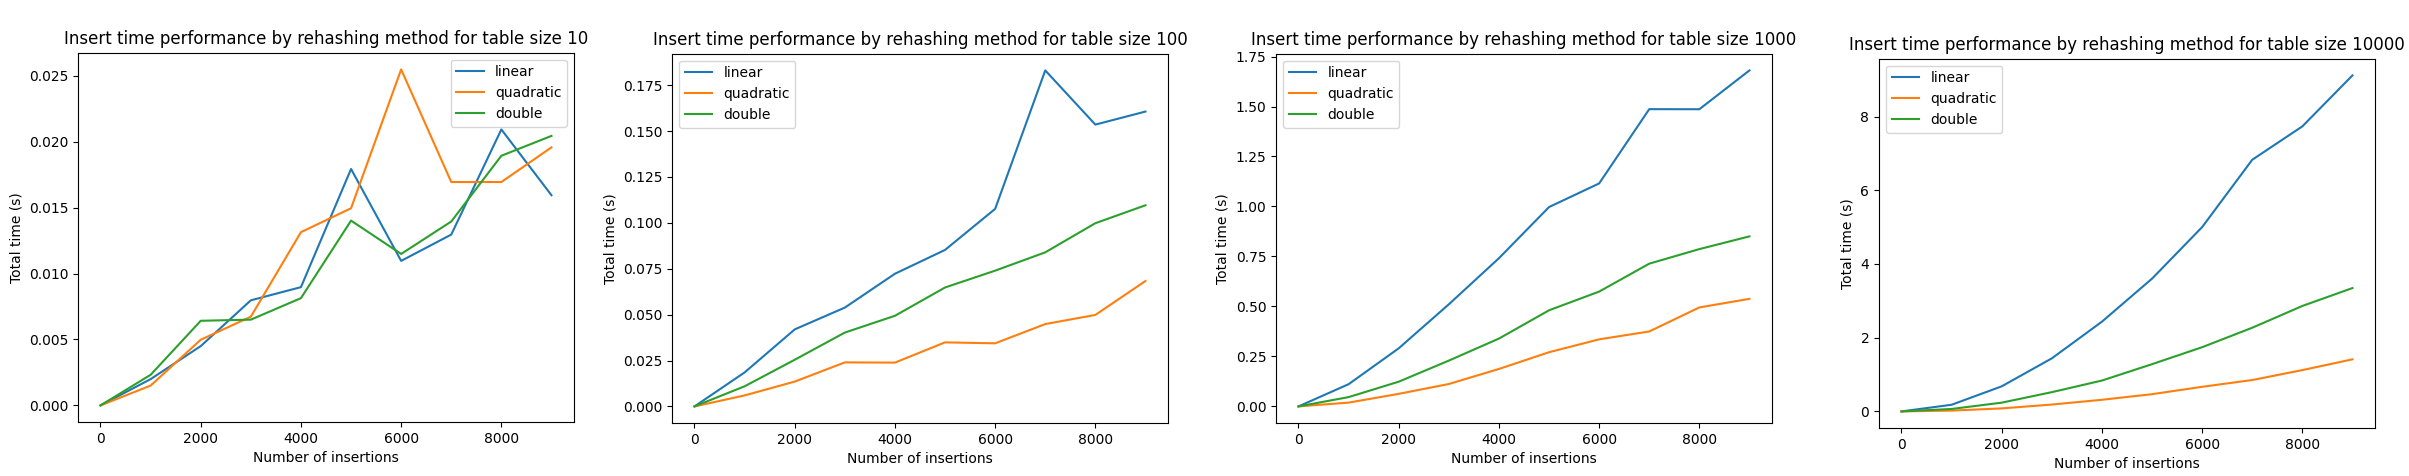
\includegraphics[width=\textwidth]{out/insert_time}
            \caption{Insertion time for different hash methods.}
            \label{fig:Insertion time}
        \end{subfigure}
        \hfill
        \begin{subfigure}
            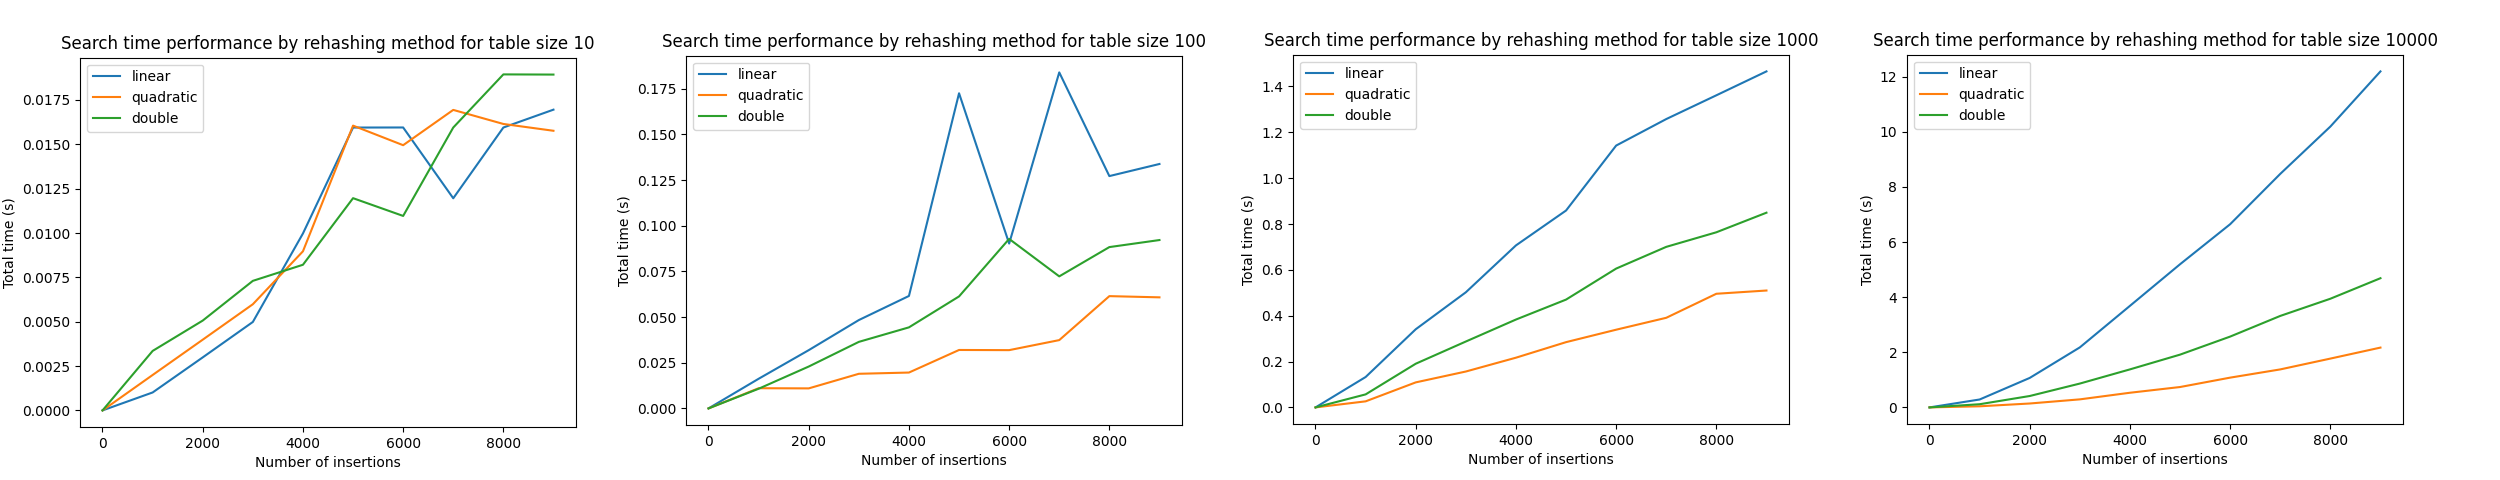
\includegraphics[width=\textwidth]{out/search_time}
            \caption{Search time for different hash methods.}
            \label{fig:Search time}
        \end{subfigure}
        \hfill
        \begin{subfigure}
            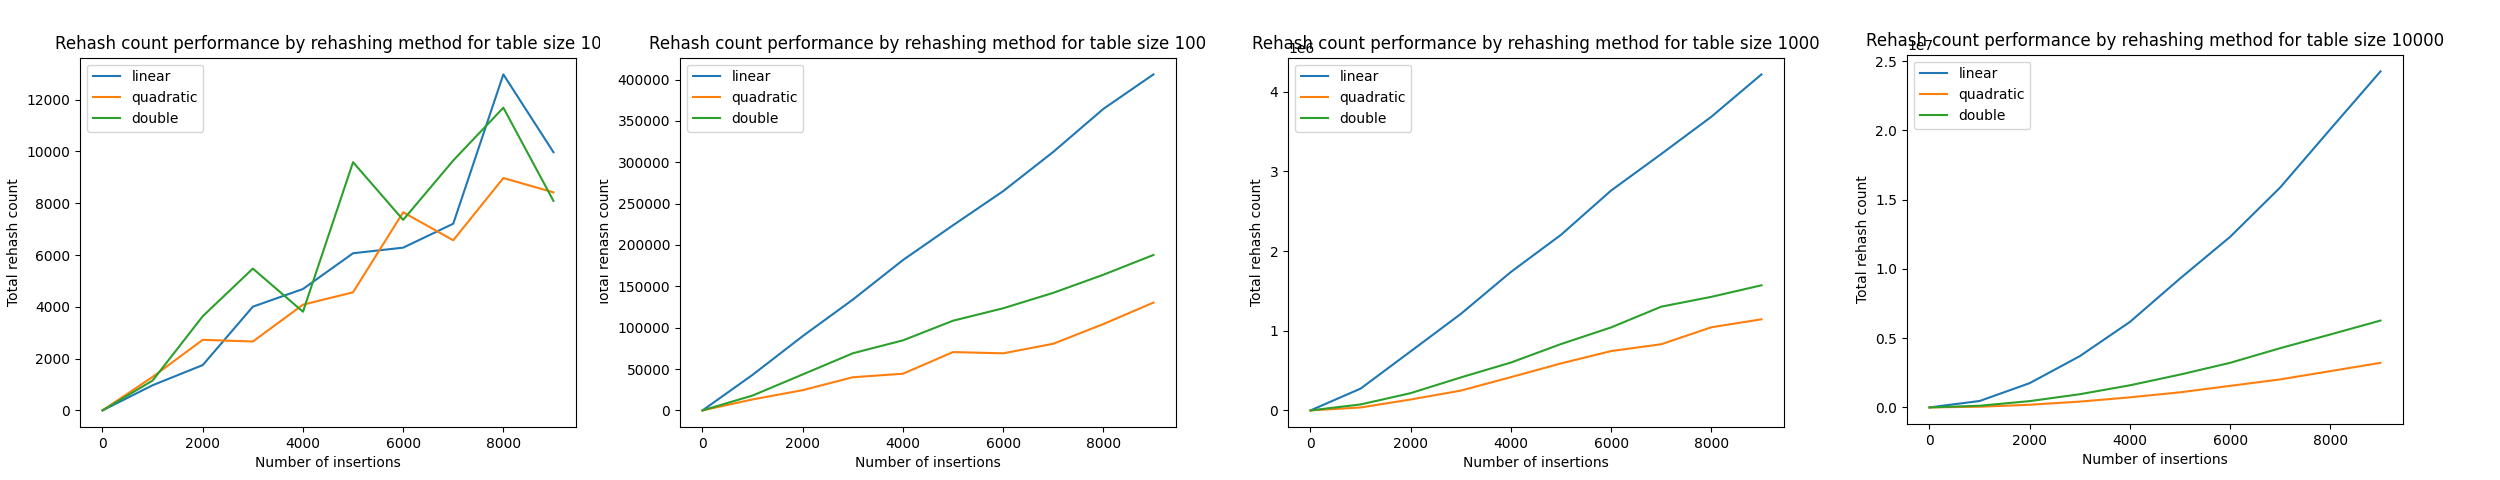
\includegraphics[width=\textwidth]{out/rehash_count}
            \caption{Rehash count for different hash methods.}
            \label{fig:Rehash count}
        \end{subfigure}
        \caption{Performances graphs.}
        \label{fig:performances graph}
    \end{figure}

    \newpage
    Les graphiques montrent que pour petites tailles de tableau, les résultats des différentes méthodes de hachage se confonde.
    En effet, pour des tailles de table de 10 ou 100, la différence de temps d'exécution entre les différentes méthodes de hachage est négligeable, qu'importe la méthode de rehachage utilisée.
    En revanche, plus la taille de la table augmente, et plus le nombre de valeurs à insérer augmente, plus les différences de temps d'exécution entre les différentes méthodes de hachage deviennent significatives.
    En effet, la méthode de hachage linéaire est la plus lente, sa courbe est relativement plate et se situe systématiquement au dessus des autres courbes.
    La courbe semble suivre être parfaitement croissante et proportionnelle aux nombres d'éléments à insérer.
    Les méthodes de hachage quadratique et double hachage sont plus rapides que la méthode linéaire, en effet leurs courbes sont moins régulières d'allure mais présente une croissance moins importante en fonction du nombre d'éléments à insérer.
    Plus la taille de la table augmente, plus ces deux méthodes se distinguent de la méthode linéaire.
    Entre ces deux méthodes, l'évolution est pratiquement similaire.
    On peut tout de même constater que la méthode de hachage quadratique est légèrement plus rapide que la méthode de hachage double.
    Cette évolution est par ailleurs progressiste : plus la taille de la table augmente, plus la méthode de hachage double se rapproche de la méthode de hachage quadratique.
    Sur l'insertion, on constate une nette différence entre les 3 méthodes : la méthode de hachage linéaire est parfaitement plate, tandis que les deux autres méthodes présentes de nombreuses imperfections dans leur courbe dûe à la présence de collisions.

    \subsection{Résultats}\label{subsec:resultats}

    Comme prévu, les résultats démontrent que les méthodes de hachage quadratique et double hachage sont plus efficaces que la méthode de hachage linéaire et de manière significative.
    Les temps d'exécutions de la méthode de hachage linéaire augmentent proportionnellement à la taille de la table et au nombre d'éléments à insérer, présentant une courbe parfaitement plate.
    Les méthodes de hachage quadratique et double hachage, quant à elles, présentent des courbes plus irrégulières, mais moins croissantes.

    Ainsi, on peut dire que la méthode de hachage quadratique est la plus viable et la plus efficace pour l'insertion, la suppression et la recherche.
    La méthode de hachage double est également efficace, mais légèrement moins que la méthode de hachage quadratique.
    En revanche, la méthode de hachage linéaire est la moins efficace, et ne devrait être utilisée que dans des cas très particuliers, où la taille de la table est très petite.

    \newpage
    \section{Complexité algorithmique}\label{sec:complexite}
    \subsection{Définition}\label{subsec:def}
    La complexité algorithmique est une mesure de la quantité de ressources (temps, mémoire, etc.) nécessaires pour exécuter un algorithme donné.
    Elle permet d'évaluer l'efficacité d'un algorithme et de comparer différentes solutions algorithmiques pour un même problème.

    Il existe deux types de complexité algorithmique : la complexité temporelle et la complexité spatiale.

    La complexité temporelle mesure le temps nécessaire à l'exécution de l'algorithme en fonction de la taille de l'entrée (par exemple, le nombre d'éléments dans un tableau).
    Elle est généralement exprimée en fonction de la notation de Landau, qui permet de caractériser la croissance de la fonction en fonction de la taille de l'entrée.
    Les notations couramment utilisées incluent O(grand O), Ω(grand omega) et Θ(grand thêta).

    La complexité spatiale mesure la quantité de mémoire nécessaire à l'exécution de l'algorithme en fonction de la taille de l'entrée.
    Elle est également exprimée en fonction de la notation de Landau.

    En général, on cherche à minimiser la complexité algorithmique pour obtenir des algorithmes efficaces qui peuvent traiter rapidement de grandes quantités de données avec un minimum de ressources.

    \subsection{Complexité de l'implémentation}\label{subsec:complexite}

    La complexité algorithmique des méthodes de rehash dépend de la méthode utilisée.

    Pour la méthode de rehash linéaire, la complexité temporelle est de O(1), car elle ne dépend pas de la taille de la table de hachage.

    Pour la méthode de rehash quadratique, la complexité temporelle est de O(1) dans le meilleur des cas (lorsqu'il n'y a pas de collisions), mais elle peut être jusqu'à O(n) dans le pire des cas (lorsque la table de hachage est remplie à capacité maximale). En moyenne, la complexité temporelle est de O(1) si la table de hachage est bien dimensionnée.

    Pour la méthode de rehash double, la complexité temporelle est de O(1) dans la plupart des cas, mais elle peut également atteindre O(n) si la table de hachage est remplie à capacité maximale.
    La complexité spatiale de cette méthode est plus élevée que celle des deux autres méthodes, car elle utilise deux fonctions de hachage.

    \newpage
    \section{Conclusion}\label{sec:conclusion}

    \subsection{Synthèse}\label{subsec:synthese}

    Dans ce projet, nous avons implémenté la classe \texttt{Table} qui permet de créer une table de hachage.
    En son sein, nous avons implémenté les méthodes de hachage linéaire, quadratique et double.
    Nous avons ensuite comparé les performances de ces méthodes en termes de temps d'exécution pour l'insertion, la suppression et la recherche.
    Nous avons également comparé les performances de ces méthodes en termes de complexité algorithmique.
    Les résultats obtenus montrent que les méthodes de hachage quadratique et double hachage sont plus efficaces que la méthode de hachage linéaire.
    La méthode de hachage linéaire est la moins efficace, et ne devrait être utilisée que dans des cas très particuliers, où la taille de la table est très petite.
    La méthode de hachage quadratique est la plus viable et la plus efficace pour l'insertion, la suppression et la recherche.
    En ce qui concerne la complexité algorithmique, on remarque que l'ensemble des méthodes de rehash ont une complexité temporelle de O(1) dans le meilleur des cas.
    En revanche, la complexité temporelle peut être jusqu'à O(n) dans le cas de la méthode de rehash quadratique et de la méthode de rehash double si la table de hachage est remplie à capacité maximale.

    \subsection{Perspectives}\label{subsec:perspectives}

    Afin d'améliorer cette étude et de l'approfondir, il serait intéressant de comparer les performances de ces méthodes de hachage avec d'autres méthodes de hachage existantes.
    Il serait également intéressant de comparer les performances de ces méthodes de hachage avec d'autres structures de données telles que les arbres binaires de recherche, les arbres AVL, les arbres B, etc.
    Enfin, il serait intéressant de comparer les performances de ces méthodes de hachage avec des algorithmes de tri tels que le tri par insertion, le tri par sélection, le tri par tas, etc.

    \subsection{limites}\label{subsec:limites}

    Les limites de cette étude sont les suivantes :
    \begin{itemize}
        \item Les méthodes de hachage implémentées ne sont pas optimisées.
        \item Nous évaluons uniquement les performances de ces méthodes de hachage en termes de temps d'exécution et de complexité algorithmique.
        \item Nous n'avons pas comparé les performances de ces méthodes de hachage avec d'autres méthodes de hachage existantes.
        \item Nous n'avons pas comparé les performances de ces méthodes de hachage avec d'autres structures de données.
        \item Nous n'avons pas comparé les performances de ces méthodes de hachage avec des algorithmes de tri.
        \item Nous n'avons pas évalué les performances de ces méthodes de hachage en termes de consommation de mémoire et ressources.
        \item Nous n'avons pas évoqué les aspects de sécurité et de confidentialité des données (attaque de collision, attaque de preuve de travail, etc.)
    \end{itemize}

    \newpage
    \section{Annexes}\label{sec:annexes}
    \subsection{Code source}\label{subsec:code}

Ci-dessous est présenté le code source de la classe \texttt{Table}.

\begin{lstlisting}[language=Python,label={lst:codesrc}]

import time
import random
from tqdm import tqdm
import matplotlib.pyplot as plt


class Table:
    def __init__(self, table_size, hash_func, rehash_type):
        """
        Constructor for Table class

        :param table_size: size of the table
        :param hash_func: hash function to use
        :param rehash_type: rehash type to use
        """
        self.table_size = table_size
        self.table = [None] * self.table_size
        self.hash_func = hash_func
        self.rehash_type = rehash_type
        self.rehash_count = 0

    def _rehash(self, key, i):
        """
        Rehash function to use for collision resolution

        :param key: key to rehash
        :param i: iteration number
        :return: rehashed key
        """
        if self.rehash_type == 'linear':
            return (key + i) % self.table_size
        elif self.rehash_type == 'quadratic':
            return (key + i * i) % self.table_size
        elif self.rehash_type == 'double':
            hash1 = key % self.table_size
            hash2 = 1 + (key % (self.table_size - 2))
            return (hash1 + i * hash2) % self.table_size

    def insert(self, key, value):
        """
        Inserts a key-value pair into the table

        :param key: key to insert
        :param value: value to insert
        :return: True if successful, False otherwise
        """
        i = 0
        while i < self.table_size:
            hashed_key = self.hash_func(key)
            rehashed_key = self._rehash(hashed_key, i)
            if self.table[rehashed_key] is None:
                self.table[rehashed_key] = (key, value)
                return True
            elif self.table[rehashed_key][0] == key:
                self.table[rehashed_key] = (key, value)
                return True
            else:
                i += 1
                self.rehash_count += 1
        return False

    def delete(self, key):
        """
        Deletes a key-value pair from the table

        :param key: key to delete
        """
        i = 0
        while i < self.table_size:
            hashed_key = self.hash_func(key)
            rehashed_key = self._rehash(hashed_key, i)
            if self.table[rehashed_key] is None:
                return
            elif self.table[rehashed_key][0] == key:
                self.table[rehashed_key] = None
                return
            else:
                i += 1
        return

    def exist(self, key):
        """
        Checks if a key exists in the table

        :param key: key to check
        :return: True if key exists, False otherwise
        """
        i = 0
        while i < self.table_size:
            hashed_key = self.hash_func(key)
            rehashed_key = self._rehash(hashed_key, i)
            if self.table[rehashed_key] is None:
                return False
            elif self.table[rehashed_key][0] == key:
                return True
            else:
                i += 1
        return False

    def value(self, key):
        """
        Returns the value associated with a key

        :param key: key to check
        :return: value associated with key
        """
        i = 0
        while i < self.table_size:
            hashed_key = self.hash_func(key)
            rehashed_key = self._rehash(hashed_key, i)
            if self.table[rehashed_key] is None:
                return None
            elif self.table[rehashed_key][0] == key:
                return self.table[rehashed_key][1]
            else:
                i += 1
        return None

    def union(self, other_table):
        """
        Returns a new table that is the union of the current table
and the other table

        :param other_table: other table to union with
        :return: new table that is the union of the current table
and the other table
        """
        # Create a new table with the same size and hash function
        # as the current table
        union_table = Table(self.table_size,self.hash_func,self.rehash_type)

        # Add all the elements from the current table to the new table
        for i in range(self.table_size):
            if self.table[i] is not None:
                union_table.insert(self.table[i][0], self.table[i][1])

        # Add all the elements from the other table to the new table
        for i in range(other_table.table_size):
            if other_table.table[i] is not None:
                union_table.insert(
                    other_table.table[i][0],
                    other_table.table[i][1]
                )

        return union_table

    def intersection(self, other_table):
        """
        Returns a new table that is the intersection
of the current table and the other table

        :param other_table: other table to intersect with
        :return: new table that is the intersection
of the current table and the other table
        """
        # Create a new table with the same size
        # and hash function as the current table
        intersection_table = Table(
            self.table_size,
            self.hash_func,
            self.rehash_type
        )

        # Add elements to the new table only if they exist in both tables
        for i in range(self.table_size):
            if self.table[i] is not None \
                and other_table.exist(self.table[i][0]):
                intersection_table.insert(
                    self.table[i][0],
                    self.table[i][1]
            )

        return intersection_table

    def display(self):
        """
        Displays the table
        """
        for i in range(self.table_size):
            print(f"{i}: {self.table[i]}")

def test_table(size=5, hash_func=lambda x: x % 5, rehash_type='linear'):
    """
    Tests the Table class

    :param size: size of table
    :param hash_func: hash function to use
    :param rehash_type: rehash function to use
    """

    # create a new table object
    table = Table(size, hash_func, rehash_type)

    # test insert method
    assert table.insert(10, "value1") is True
    assert table.insert(5, "value2") is True
    assert table.insert(20, "value3") is True

    # test exist method
    assert table.exist(10) is True
    assert table.exist(5) is True
    assert table.exist(20) is True
    assert table.exist(15) is False

    # test value method
    assert table.value(10) is "value1"
    assert table.value(5) is "value2"
    assert table.value(20) is "value3"
    assert table.value(15) is None

    # test delete method
    table.delete(10)
    assert table.exist(10) is False
    assert table.value(10) is None

    # create another table object
    other_table = Table(size, hash_func, rehash_type)
    other_table.insert(5, "other_value1")
    other_table.insert(15, "other_value2")
    other_table.insert(25, "other_value3")

    # test union method
    union_table = table.union(other_table)
    assert union_table.exist(5) is True
    assert union_table.exist(15) is True
    assert union_table.exist(20) is True
    assert union_table.exist(25) is True

    # test intersection method
    intersection_table = table.intersection(other_table)
    assert intersection_table.exist(5) is True
    assert intersection_table.exist(15) is False
    assert intersection_table.exist(20) is False
    assert intersection_table.exist(25) is False

    # test display method
    table.display()

test_table(5, lambda x: x % 5, 'linear')

result = {
    'linear': {},
    'quadratic': {},
    'double': {}
}

def test_rehashing(n, rehash_type='linear', table_size=100):
    """
    test the Table class with rehashing

    :param n: number of elements to insert
    :param rehash_type: rehash function to use
    """

    # Create a table with size 10
    table = Table(table_size, lambda x: x % 10, rehash_type)

    # Insert n random elements
    insert_start_time = time.time()
    for i in range(n):
        key = random.randint(0, 100)
        value = i
        table.insert(key, value)
    insert_end_time = time.time()

    # Time the search for all n elements
    search_start_time = time.time()
    for i in range(n):
        key = random.randint(0, 100)
        table.value(key)
    search_end_time = time.time()

    result[rehash_type].update({
        n: {
            'table_size': table.table_size,
            'number_of_elements': n,
            'search_time': search_end_time - search_start_time,
            'insert_time': insert_end_time - insert_start_time,
            'average_time_per_search':
                (search_end_time - search_start_time) / n,
            'rehash_count': table.rehash_count,
        }
    })

for table_size in [10, 100, 1000, 5000, 10000, 50000, 100000]:

    list_rehash_types = ['linear', 'quadratic', 'double']
    for rehash_type in list_rehash_types:
        for i in tqdm(
            range(1, 100000, 1000),
            desc=f'Progress for {rehash_type} rehashing \
            with table size {table_size}'):

            test_rehashing(i, rehash_type, table_size)

    linear_data = []
    quadratic_data = []
    double_data = []

    for method in ['linear', 'quadratic', 'double']:
        data = []
        for key in range(1, 100000, 1000):
            data.append([
                key, result[method][key]['number_of_elements'],
                result[method][key]['search_time'],
                result[method][key]['insert_time'],
                result[method][key]['rehash_count']
            ])
        if method == 'linear':
            linear_data = data
        elif method == 'quadratic':
            quadratic_data = data
        elif method == 'double':
            double_data = data

        plt.plot(
        [x[1] for x in linear_data],
        [x[2] for x in linear_data],
        label='linear')
    plt.plot(
        [x[1] for x in quadratic_data],
        [x[2] for x in quadratic_data],
        label='quadratic')
    plt.plot(
        [x[1] for x in double_data],
        [x[2] for x in double_data],
        label='double')

    plt.xlabel('Number of insertions')
    plt.ylabel('Total time (s)')
    plt.title(f'Search time performance by rehashing method \
        for table size {table_size}')
    plt.legend()
    plt.show()

    plt.plot(
        [x[1] for x in linear_data],
        [x[3] for x in linear_data],
        label='linear')
    plt.plot(
        [x[1] for x in quadratic_data],
        [x[3] for x in quadratic_data],
        label='quadratic')
    plt.plot(
        [x[1] for x in double_data],
        [x[3] for x in double_data],
        label='double')

    plt.xlabel('Number of insertions')
    plt.ylabel('Total time (s)')
    plt.title(f'Insert time performance by rehashing method \
        for table size {table_size}')
    plt.legend()
    plt.show()

    plt.plot(
        [x[1] for x in linear_data],
        [x[4] for x in linear_data],
        label='linear')
    plt.plot(
        [x[1] for x in quadratic_data],
        [x[4] for x in quadratic_data],
        label='quadratic')
    plt.plot(
        [x[1] for x in double_data],
        [x[4] for x in double_data],
        label='double')

    plt.xlabel('Number of insertions')
    plt.ylabel('Total rehash count')
    plt.title(f'Rehash count performance by rehashing method \
        for table size {table_size}')
    plt.legend()
    plt.show()

\end{lstlisting}
\end{document}





